\documentclass[quiet, 10pt, letterpaper]{l3doc}
\usepackage{pdfpages}
\AddToHook{env/function/before}{\vspace*{-.6\baselineskip}}
\AddToHook{env/syntax/after}{\par\vspace*{.1\baselineskip}}
\def \TFF {true\textbar \textbf{false}}
\def \TTF {\textbf{true}\textbar false}
\setlength \parindent {0pt}
\setlist[description]{leftmargin = 0pt}
\def \key #1{\textcolor{red}{\textbf{\texttt{#1}}}}
\def \keyval #1#2{\key{#1} \normalfont \texttt{=} \meta{\textup{#2}}}
\usepackage{ctex}
\setCJKmainfont{LXGW WenKai}
\setCJKsansfont{LXGW Marker Gothic}

\title{^^X
  \sffamily \cls{litetable} 文档类 -- 多彩的课程表\thanks
    {^^X
      \url{https://github.com/myhsia/litetable},
      \url{https://ctan.org/pkg/litetable}
    }
}
\author{^^X
  夏明宇 \texttt{<\href{mailto:myhsia@outlook.com}{myhsia@outlook.com}>}^^X
  \thanks{
    \href{https://github.com/ljguo1020}{郭李军}
    开发了读取 \meta{left} \cmd{->} \meta{right} 型数据结构的接口,
    并为低版本 \hologo{TeX} Live 做兼容.
  }
}
\date{Released 2025-02-10\quad \texttt{v3.2A}}

\begin{document}

\maketitle

\section{介绍}

\cls{litetable} 文档类提供了一个多彩的课程表设计,
基于 \cls{article} 和 \pkg{tikz} 由 \pkg{expl3} 开发.
其兼容发行版 \hologo{TeX} Live 2019 及更高版本,
支持 \hologo{pdfLaTeX},\hologo{XeLaTeX} 和 \hologo{LuaLaTeX} 等多种编译方式.
点击跳转至手册的
\href{http://mirrors.ctan.org/macros/latex/contrib/^^X
  litetable/doc/litetable-en-us.pdf^^X
}{[\textsf{English Version}]}
\href{http://mirrors.ctan.org/macros/latex/contrib/^^X
  litetable/doc/litetable-zh-hk.pdf^^X
}{[\textsf{粵語版本}]}.

\section{用户接口}

\DescribeEnv{litetable}
此环境可生成一个空白课程表框架,
需在命令 \cs{timelist},\cs{weeklist} 后执行
\begin{quote}
  |\begin{litetable}|
    \oarg{keys} \marg{title} \oarg{keys}| ... |^^X
  |\end{litetable}|
\end{quote}
强制参数用于设定课程表标题,
可选参数接受以下键
\begin{description}
  \item [\keyval{color}{color}] 可设置课程表框架的背景色,
  默认值为 \cmd{gray}. 键名可省略.
  \item [\keyval{sem}{string}]
  可设置页面右上角的学期信息.
\end{description}

\begin{function}{\weeklist}
  \begin{syntax}
    \cs{weeklist} \oarg{keys} \marg{list} \oarg{keys}
  \end{syntax}
  强制参数接收数组,
  用于设置课程表顶部的工作日列表和列宽.
  可选参数接受以下键
  \begin{description}
    \item [\keyval{format}{format commands}]
    可设置工作日列表格式,默认为 \cmd{\bfseries}\cmd{\scshape}.
    \item [\keyval{sep}{string}] 可设置工作日列表的分隔符,
    默认为空.
  \end{description}
  \begin{verbatim}
    \weeklist [ format = \bfseries \scshape, sep = \textbar ]
      { Mon -> 1, Tue -> 1, Wed -> 1, Thu -> 1, Fri -> 1 }
  \end{verbatim}
\end{function}

\begin{function}{\timelist}
  \begin{syntax}
    \cs{timelist} \oarg{keys} \marg{list} \oarg{keys}
  \end{syntax}
  强制参数均接收数组,用于设置课程表的左侧的时间列表.
  可选参数接受以下键
  \begin{description}
    \item [\keyval{numformat}{format}]
    可设置时间列表的序号字体,
    默认为 \cmd{\ttfamily}\cmd{\bfseries}.
    \item [\keyval{timefont}{format}] 可设置时间列表的时间字体,
    默认为 \cmd{\ttfamily}.
    \item [\keyval{hidetime}\TFF] 用于隐藏时间列表中的时间,只保留序号.
    初始为 \cmd{false}.
  \end{description}
  \begin{verbatim}
    \timelist [ numformat = \bfseries, timeformat = \ttfamily ]
      { 08:30 -> 10:00, 10:30 -> 12:00, 13:00 -> 14:30, 15:00 -> 16:30 }
  \end{verbatim}
\end{function}

\begin{function}{\course}
  \begin{syntax}
    \cs{course} \oarg{keys} \marg{start} \oarg{keys} \marg{end} \oarg{keys}
  \end{syntax}
  用于在当前工作日添加课程盒子,
  需在 \env{litetable} 环境中执行.
  两个强制参数分别用于设置课程的开始和结束序号.
  可选参数接收下列键
  \begin{description}
    \item [\keyval{color}{color}] 用于设置课程盒子的颜色,
    默认为 \cmd{teal}. 键名可省略.
    \item [\keyval{subject}{string}] 用于设置课程名称.
    \item [\keyval{location}{string}] 用于设置课程地点.
    \item [\keyval{lecture}{string}] 用于设置授课教师.
    \item [\keyval{comment}{string}] 用于给课程添加脚注.
  \end{description}
  \begin{texnote}
    \begin{itemize}
      \item 若 \meta{start} \cmd{=} \meta{end},即课程盒子的高度为 1,
      则 \key{location} 和 \key{lecture} 将输出在同一行,
      \key{comment} 的值将会隐藏.
      \item 即使误将 \meta{start} 与 \meta{end} 写反,
      模板也会自动纠正.
      \item 若 \key{location} \key{lecture} 均未使用,
      则 \key{subject} 将输出在课程盒子中心.
      \item 超出课程表范围的课程盒子将不显示,
      并会返回警告.
      输入用例见 Appendix \ref{mwe}.
    \end{itemize}
  \end{texnote}
\end{function}

\begin{function}{\newday}
  \begin{syntax}
    \cs{newday} \oarg{integral value}
  \end{syntax}
  使其后面添加的课程盒子后移 \meta{intergal value} 个工作日.
  可选参数的默认值为 \cmd{1}.
\end{function}

\begin{function}{\more}
  \begin{syntax}
    \cs{more} \marg{comment}
  \end{syntax}
  在课程表的右下角添加备注.
\end{function}

\clearpage \appendix

\section{工作示例} \label{mwe} \linespread{1.25}

\verbatiminput{litetable-demo.tex}

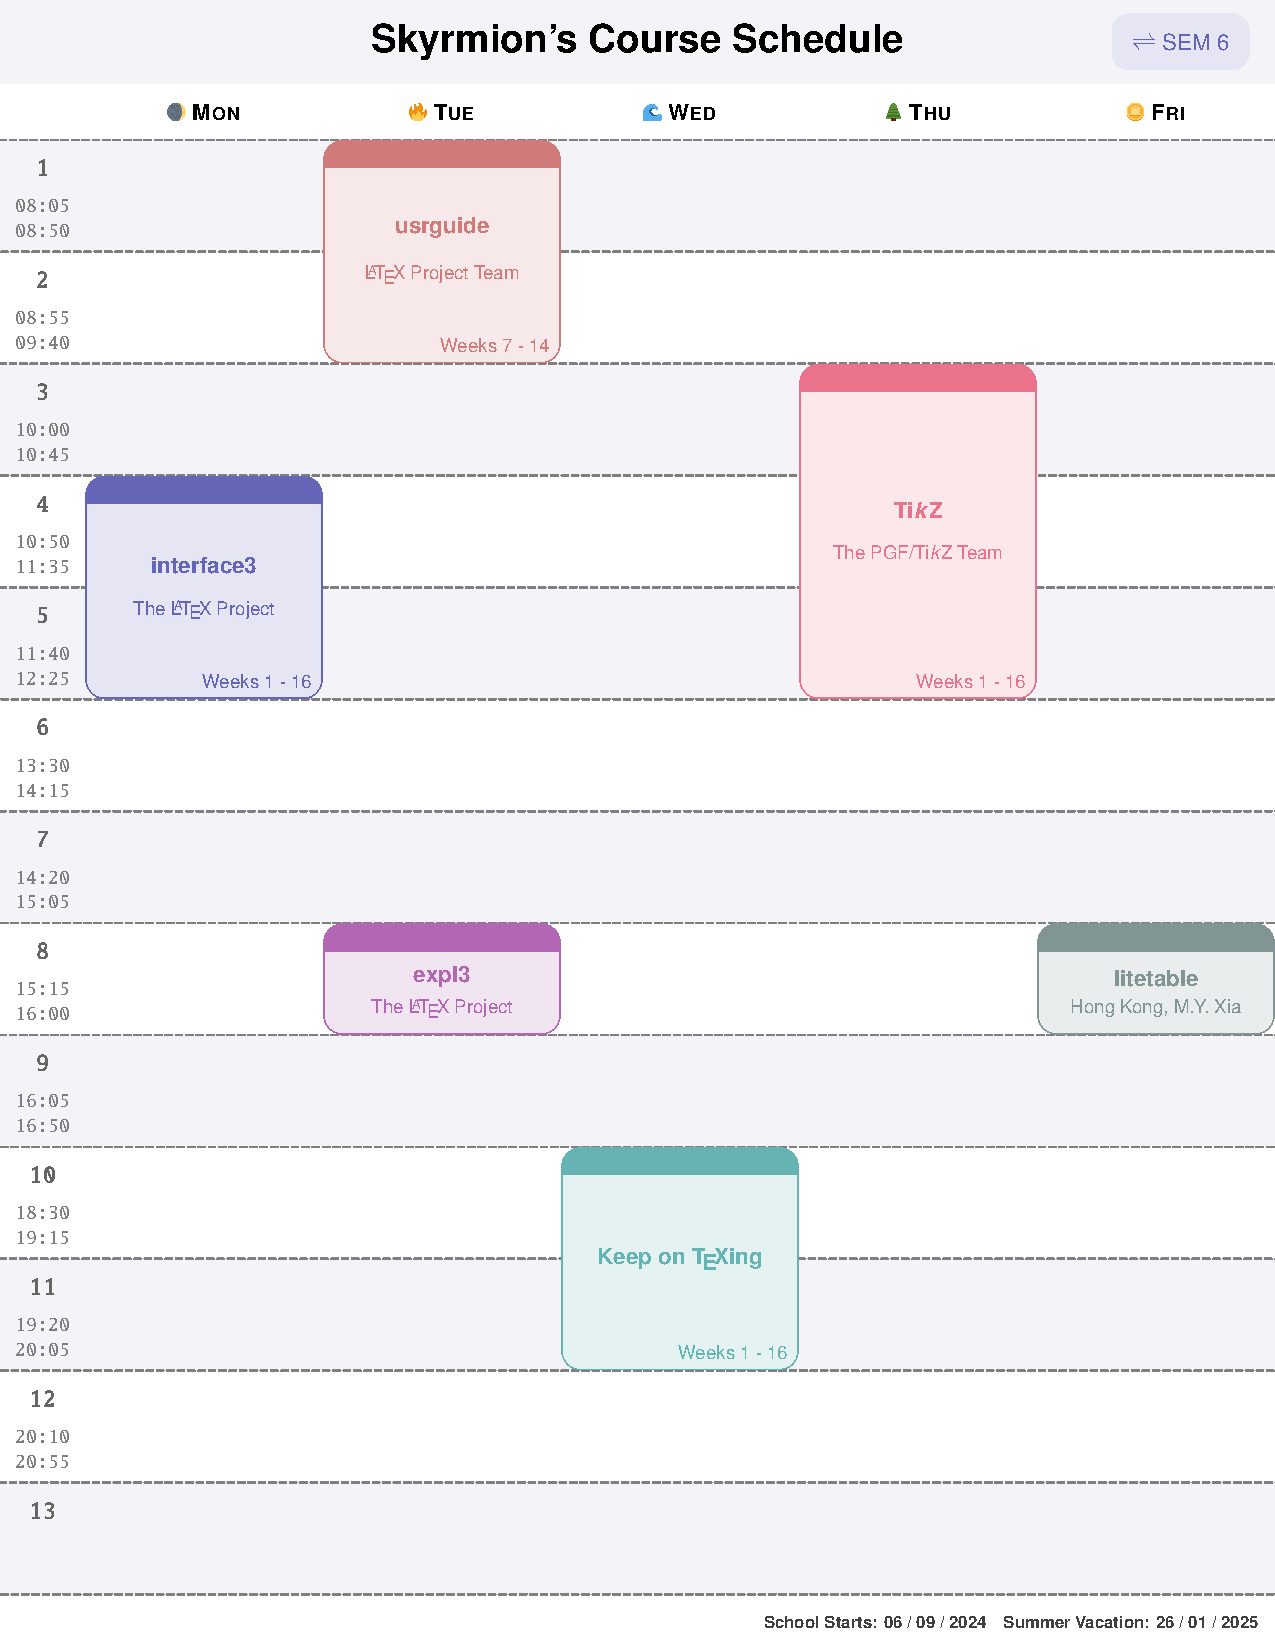
\includepdf[pages = 1]{litetable-demo.pdf}

\end{document}

% End of file litetable-zh-cn.tex
